\documentclass[aps,showpacs,twocolumn,floatfix,prx,superscriptaddress]{revtex4-1}
\usepackage{graphicx}
\usepackage{amsfonts}
\usepackage{amsmath}
\usepackage{amssymb}
\usepackage{upgreek}
\usepackage[usenames,dvipsnames]{color}

%\bibliographystyle{apsrev}


\def\s{\sigma}
\begin{document}

\title{From Brownian bridges and Fermi--Dirac statistics to exactly solvable dynamics of polymer loops.}

\author{Wenwen Huang}
\author{Yen Ting Lin}
\author{Daniela Fr\"{o}mberg}
\author{Jaeoh Shin}
%\affiliation{Max Planck Institute for the Physics of Complex Systems, N\"{o}thnitzer Str. 38, D-01187 Dresden, Germany}
%\author{Petrina Delivani}
%\author{Mariola Chac\'{o}n}
%\affiliation{Max Planck Institute of Molecular Cell Biology and Genetics, Pfotenhauerstrasse 108, D-01307 Dresden, Germany}
%\author{Iva M. Toli\'{c}}
%\affiliation{Max Planck Institute of Molecular Cell Biology and Genetics, Pfotenhauerstrasse 108, D-01307 Dresden, Germany}
%\affiliation{Division of Molecular Biology, Ruder Bo\v{s}kovi\'{c} Institute, Bijeni\v{c}ka cesta 54, 10000 Zagreb, Croatia}
\author{Frank J\"{u}licher}
\author{Vasily Zaburdaev}
\affiliation{Max Planck Institute for the Physics of Complex Systems, N\"{o}thnitzer Str. 38, D-01187 Dresden, Germany}


\begin{abstract}
{Very often complex biological phenomena lead to a gold mine of statistical physics problems. In this article, we show how by reformulating the problem of chromosomal loop oscillations in the language of Brownian bridges we can unfold it into a set of related models from different fields of statistical physics and analytically solve them by essentially the same approach. We first demonstrate that in one dimension a pinned polymer loop in an external force field can be approximated by a combination of Brownian bridge and Fermi-Dirac statistics, while the exact solution can be obtained via the fermion integer partition problem. Next analogy we explore is to the asymmetric simple exclusion process (ASEP) with reflecting boundaries. With the help of the generalized Bethe-ansatz we are able to analytically solve for its time evolution and thus gain access to the relaxation times of the system. Finally, in a way of demonstrating the results of such unexpected interplay of analogies, we show that thus calculated relaxation times of the ASEP model can be used to quantify non-equilibrium dynamics of the three-dimensional polymer loop. Thus we provide a unifying theoretical approach to a set of prototypical models of statistical physics which are of a broad interest to the fields of polymer physics, number theory, exclusion processes and single-file diffusion.}
\end{abstract}
\maketitle


\section{Introduction}
Through the decades of DNA research it has been demonstrated that simple polymer models are extremely powerful tools to quantify various biological phenomena involving dynamics and statistics of DNA molecules: from {\em in vivo} mechanical properties of stretched DNA strands \cite{} to {\em in vitro} chromosomal territories \cite{}, and hiC data \cite{}. Simple models, like the freely jointed chain or random coil model \cite{}, often combine analytical tractability and predictive power. Recently we have considered a problem of chromosome alignment by the drag forces during meiosis in fission yeast \cite{}. In polymer language this problem can be reformulated as finding the statistics of a pinned polymer loop in a uniform external force field. By mapping the original biological question to essentially a random walk problem we could solve for statistics of chromosomes in a quite complex three-dimensional geometry with constraints. However, the developed theory only delivered predictions for the equilibrium setting, while leaving the dynamics of the process beyond its reach. %In a natural step towards understanding dynamics we decided first to consider the simplest realization of the one-dimensional system that lead to a series of interesting results.

In this paper, we show how the one-dimensional version of the pinned polymer loop problem serves as a starting point of a chain of unexpected analogies that interlink several fields of statistical physics. A synergy of the Brownian bridge theory and Fermi-Dirac statistics serves as an asymptotic approximation of the polymer loop statistics. However, exact solution can be found by solving the fermion number partition problem. We next notice that the dynamics of the pinned polymer loop in an external force field can be mapped to an ASEP model with reflecting boundary conditions. Via this link we can, on the one hand, immediately solve for the equilibrium statistics of the ASEP model and, on the other hand, investigate the dynamics of the polymer loop by means of the ASEP approach. Remarkably, the dynamics of the ASEP model can be solved exactly via the generalized Bethe-ansatz. We find analytical predictions for the relaxation times of the system and use them to quantify the relaxation dynamics of the three-dimensional polymer loop as a function of the external force. We test all analytical results with extensive kinetic Monte-Carlo and 3D Brownian dynamics simulations. 

Our results only cover the simplest geometries, but as highlighted by the chromosome alignment problem [], they can be naturally generalized to include further additional constraints. The interrelation of various prototypical statistical physics models, which we describe here, also implies that methods developed for a particular problem can be ported to the other ``relative'' models as well. We thus think that the theoretical results presented here will be of interest to a broad and interdisciplinary scientific community working in the fields of polymer physics, number theory, and non-equilibrium statistical physics in general. 

The manuscript is organized as follows. The next Section II is devoted to the polymer loop model and its equilibrium solution by a Brownian bridge theory and relation to the integer number partition theory in one dimension. We then turn to the dynamics and the ASEP framework in Sec.III. In Sec.IV, we illustrate how the ASEP model can be utilized to study the polymer relaxation dynamics. The last Section is reserved for the discussion and conclusions.

\section{Statistics of the one-dimensional pinned polymer loop}
A polymer loop is a ubiquitous subject in polymer research pertinent to many
important biological phenomena \cite{}. For example, fission yeast uses the
viscous drag force to suppress fluctuations and align chromosomes for
recombination by pulling on chromosomes arranged in a loop \cite{}. For a constant
pulling speed this setting is equivalent to a pinned polymer loop in the uniform
external force field \cite{}, see Fig 1a. We start by setting up a one dimensional model of
this process, see Fig. \ref{fig:schematic} for a sketch. 
\begin{figure}[htpb]
    \centering
    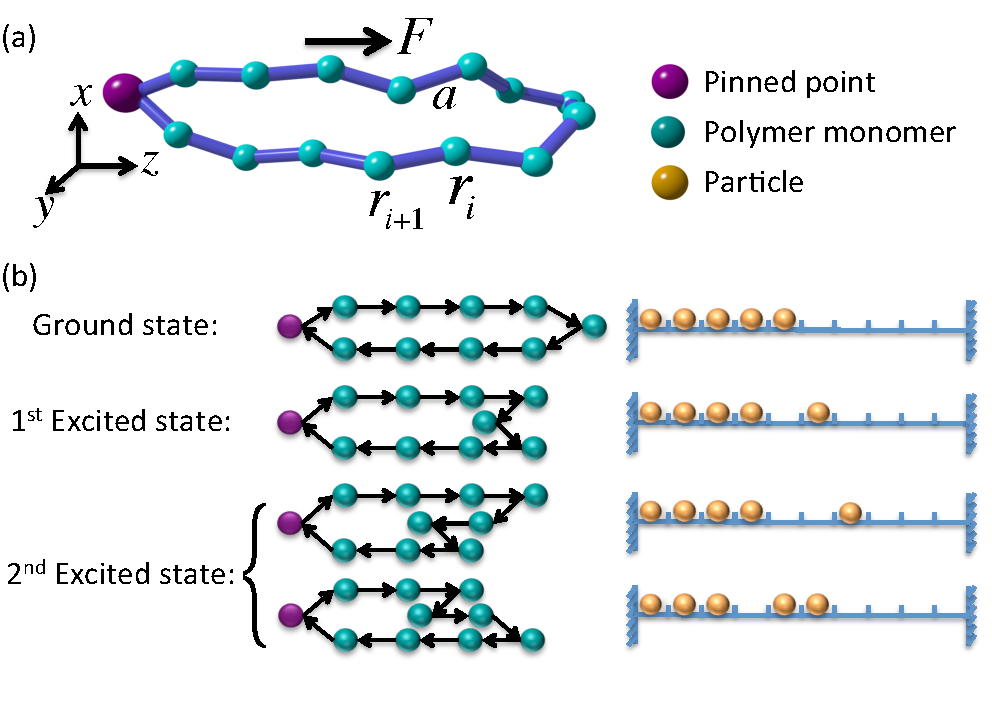
\includegraphics[width=1.0\linewidth]{schematic}
    \caption{Schematic figure for the model.}
    \label{fig:schematic}
\end{figure}


We consider a classical freely jointed chain model consisting of $L$ beads connected by $L$ rods; the rod length corresponds to the Kuhn length $a$ of the polymer. The position of the $i^{\rm th}$ bead is denoted by $z_i$, $i\in\{0,1, \ldots,L\}$. The looping condition suggests $z_0=z_L=0$. A constant external force $F$ acts on every bead (except of the pinned one) and points in the positive direction of the $z$-axis.  We define the orientation of the $i^{\rm th}$ rod as $e_j:=(z_{j+1} - z_{j})/a$ and therefore $z_i =
a\sum_{j=0}^{i} e_j$ where $e_j=\pm 1$ and $i,j \in \left\{0, 1, \ldots,
    L-1\right\}$. In addition to regular forces, there are random forces acting on the chain. We will quantify their effect by an effective temperature $T$. We do not consider the volume exclusion effects and bending
energy in this model.

Note that in the absence of force this model is equivalent to a trajectory of a one-dimensional unbiased random walk consisting of $L$ steps, where each step corresponds to a monomer (rod) in the chain. This random walk, however, has to start and end at the same point to fulfil the loop constraint. In mathematics, it is known as the Brownian bridge problem and can be solved to find the statistics of every bead position to be Gaussian with its variance depending on the number of the bead in the chain \cite{}. Therefore we can outline the strategy of solving the problem with a non-zero force: first find how the statistics of random walk steps changes in the presence of force and then enforce the Brownian bridge condition to form a loop. 

To find the statistics of random walk steps (rod orientations) we write down the potential energy of the system:
\begin{equation}
    \label{eq:energy_polymer}
    E  = -\sum_{i=0}^{L-1} {Fz_i} = -Fa\sum_{i=0}^{L-1} \sum_{j=0}^{i}e_j, 
\end{equation}
%In addition, the looping condition gives
%\begin{equation}
%    \label{eq:looping}
%    \sum_{j=0}^{L-1} e_j = 0.
%\end{equation}
We now map the polymer model to a particle system. Note that the state of rod
orientation is binary, $e_j \in \left\{-1, +1\right\}$. We can map it to the state $Z_j$ of a
lattice site $j$, which is either occupied by a particle, $Z_j = 1$, when the rod points along the force
or empty, $Z_j = 0$, if the rod points against the force, see Fig. 1b. The relation between $Z_j$ and $e_j$ is defined by a simple
variable transformation $Z_j := \left(e_j+1\right)/2$. The actual positions of polymer
beads are obtained by the back transformation
\begin{equation}
    \label{eq:z2x}
    z_i = a \sum_{j=0}^{i}{e_j} = a\left(2\sum_{j=0}^{i}{Z_j} -i\right).
\end{equation}
%Several examples of polymer configurations maps to particles on lattice sites are given
%in Fig. \ref{fig:schematic}. It is not difficult to see the boundary condition of
%lattice for the particle hopping model is reflecting boundaries. We will
%discuss more about this in section \ref{sec:asep}.
By exchanging the order of the double summation in Eq.
\eqref{eq:energy_polymer} and utilizing the loop condition  $\sum_{j=0}^{L-1} e_j = 0$ we 
arrive at 
\begin{equation}
    \label{eq:energy_particle}
    E = \tilde{E} + \Delta E \sum_{j=0}^{L-1} j Z_j, 
\end{equation}
where $\tilde{E}=  -L(L-1) \Delta E /4$ {\color{red} double check!} and $\Delta E = 2Fa$. The loop condition
implies a hard constraint of the total number of the particles
$\sum_{j=0}^{L-1} Z_j = L/2$ (there has to be equal number of steps along and against the force field to return to the origin).

\subsection{Fermi-Dirac statistics of rod orientations}
In the energy expression \eqref{eq:energy_particle} one can immediately recognize
the energy of a system of $L/2$ fermions distributed over
$L$ equidistant energy levels $0, \Delta E, \ldots, (L-1) \Delta E$, where
$Z_j$ can be interpreted as an occupation number. Clearly the lowest energy of the system corresponds to $Z_j = 1$ for $j < L/2$ and
$Z_j=0$ otherwise (fully stretched polymer loop), see Fig 1b. However, when the system is in contact with the thermal bath
at temperature $T>0$, it is possible to find other configurations. The equilibrium
Gibbs measure defines the probability of the system to be in a certain configuration via the corresponding exponential Boltzmann factor.
%$\left\{Z_j\right\}_{j=0}^{L-1}$ is
%\begin{equation}
%    \label{eq:gibbs}
%    \mathbb{P}\left\{\left\{Z_j\right\}_{j=0}^{L-1}\right\} \propto \exp
%    \left[-\frac{\Delta E \sum_{j=0}^{L-1} j Z_j}{k_B T}\right]
%\end{equation}
%where $k_B$ is the Boltzmann constant. 
Interestingly, there are two possibilities to calculate those probabilities. 


The fixed total number or particles ($L/2$) corresponds to a picture of the
\emph{canonical ensemble} \cite{Chandler1987,Huang2001}: the system does not exchange particles with
its environment. However, the technical difficulty here is in finding all degenerate microscopic states corresponding to the given total energy of the system. Before venturing in this calculation we first look at the alternative, approximate solution.

%While formally the equilibrium distribution is solved by
%\eqref{eq:gibbs}. But here the difficulty of obtaining the analytic solution due
%to the degeneracy of the system, i.e., some (total) energy levels contain
%multiple microscopic states. 

An alternative approach is to relax the fixed-number constraint, and use
the \emph{grand canonical ensemble}, which allows exchange of particles with
an external reservoir \cite{Chandler1987,Huang2001}, derive the probability
distribution of the microscopic states to construct a random walk model, and
then finally use the Brownian bridge condition to re-enforce the fixed-number constraint
\cite{Lin2015}. Under these assumptions, the statistics of the particles is now given by a solution to the standard fermionic problem.
The probability distribution of $Z_j$  is the {\em Fermi--Dirac} distribution:
\cite{Chandler1987,Lin2015}
\begin{subequations}
    \label{eq:discrete_prob}
    \begin{align}
        \mathbb{P} \left\{ Z_j = 1\right\} & =  \left\{1+\exp\left[\frac{ \Delta
                    E \left(j - \mu \right) }{k_B T}\right]\right\}^{-1}, \\
        \mathbb{P} \left\{ Z_j = 0\right\} & = 1 - \mathbb{P} \left\{ Z_j =
            1\right\},
    \end{align}
\end{subequations}
with a chemical potential $\mu = (L+1)/2$ {\color{red} check!} obtained from the requirement that on average there are $L/2$ particles in the system.
Noting the relation of $Z_j$ and the orientation of $j^{\rm
    th}$ rod $e_j = \left(2Z_j -1\right)$, the probabilities
\eqref{eq:discrete_prob} can be used to compute the distribution of $e_j$. The Fermi--Dirac distribution shows that in the presence of the external force field the first half of the steps is biased in the direction of force, whereas the second half of steps has higher probability of pointing against the force field.
%In this
%context, the famous Pauli exclusion principle---$Z_j$ can be either $0$ or
%$1$---corresponds to an almost trivial statement of each rod: either it points to
%the right ($Z_j=1$) or to the left ($Z_j=0$).  
We emphasize that only in the
picture of the grand canonical ensemble, the probability distributions of each rod orientation
are mutually independent.%; with a hard constraint of the particle number, $Z_j$'s
%are not independently distributed. In fact, the independence is the key for an
%analytic solutions of the equilibrium properties, such as \eqref{eq:gibbs}, are
%possible. 

Given the probability distribution of the occupation number (rod orientation), their mean
and variance can be easily
calculated:
\begin{subequations}
    \begin{align}
        \label{eq:zmean}
        \mathbb{E}\left[Z_j\right] & =  \mathbb{P} \left\{ Z_j = 1\right\} ,\\
        \label{eq:zvar}
        \text{var}\left[Z_j\right] & = \mathbb{P} \left\{ Z_j = 1\right\} \cdot
        \left( 1 - \mathbb{P} \left\{ Z_j = 1\right\} \right) -
        \mathbb{E}\left[Z_j\right]^2.
    \end{align}
\end{subequations}
Now that we know the statistics of individual steps we can construct the corresponding random walk process. Let us look at its trajectory connecting beads $k$ and $l$, $l>k$ and the corresponding propagator $\rho(z_l=z|z_k=0)$. Remarkably, according to the Lindeberg-Feller central limit theorem \cite{} this propagator is  Gaussian with the mean and variance equal to the sum of mean and variance of all individual steps leading from bead $k$ to $l$. We therefore found the statistics of random walks governing the polymer loop in the presence of the external force field. However, due to the grand canonical approach, such random walks would return to the origin only on average. While this random walk properly reproduces the mean position of every bead, but it is not able to predict the fluctuations of bead position. To work out the variance of the bead position we have to enforce the loop condition.
 
%With \eqref{eq:zmean}, \eqref{eq:zvar}, a random walk is then built, satisfying
%the first and the second moments of the individual rods. Specifically, we
%construct a Gaussian random walk, which satisfies the conditional probability
%\begin{equation}
%    \label{eq:xmean}
%    \rho\left(z_{i+1} \vert z_i\right) =\exp\left\{ -\frac{\left[z_{i+1}- z_i -
%                a\mathbb{E}\left[Z_j\right]\right]^2}{4
%            \text{var}\left[Z_j\right]a^2}\right\}, 
%\end{equation}
%on a continuum domain $z \in \mathbb{R}$. 
\subsection{Imposing the Brownian bridge condition}
The Brownian bridge condition is a straightforward formulation of the condition that a bead with an index $i$ is a part of the loop of length $L$. The bead $i$ belongs to the loop if two pieces of random walk trajectory of length $i$ and $L-i$ respectively can meet at the position of the bead and belong to the same loop. Thus the probability density function of finding the bead in a given coordinate $z$ is given by
\begin{equation}
    \label{eq:bridge}
    \rho^L\left(z_i = z\right) = \frac{\rho\left(z_i = z \vert z_0 = 0\right)
        \rho\left(z_{L-i} = z \vert z_L = 0\right)}{\rho\left(z_L = 0 \vert z_0
            = 0\right)},
\end{equation}
where $ \rho\left(z_k = z \vert z_j = 0\right)$ are the propagators of the corresponding random walk process. In case of the pinned polymer loop those propagators are Gaussian distributions with a mean and variance obtained as a sum of means and variances of all contributing individual steps of the random walk. Importantly, because each propagator entering the above Eq.(\ref{eq:bridge}) is Gaussian, the resulting $\rho^L\left(z_i = z\right)$ is Gaussian as well. Its variance is given by
\begin{equation}
    \label{eq:bridgeVar}
    \text{var}\left[z_i^L\right] =
    \frac{\sum_{j=0}^i\text{var}\left[Z_j\right]\sum_{j=L-i}^L\text{var}\left[Z_j\right]}{\sum_{j=0}^L\text{var}\left[Z_j\right]}
\end{equation}
We can now use these results and compare with direct Monte-Carlo simulations of
the one-dimensional pinned polymer loop in the external force field. In Fig.
\ref{fig:meanVar} we plot the mean (a) and variance (b) of every bead position for different strengths of the external force field. With increasing force the polymer becomes more stretched and fluctuations decrease. In the limit of zero force we recover the well known result of the standard Brownian bridge problem \cite{}. Although calculating the sums involved in the estimation of the mean and variance does not present any particular difficulty, for not too small temperatures the sums can be approximated by integrals and evaluated explicitly (see Appendix A for details). 
\begin{figure}[htpb]
    \centering
    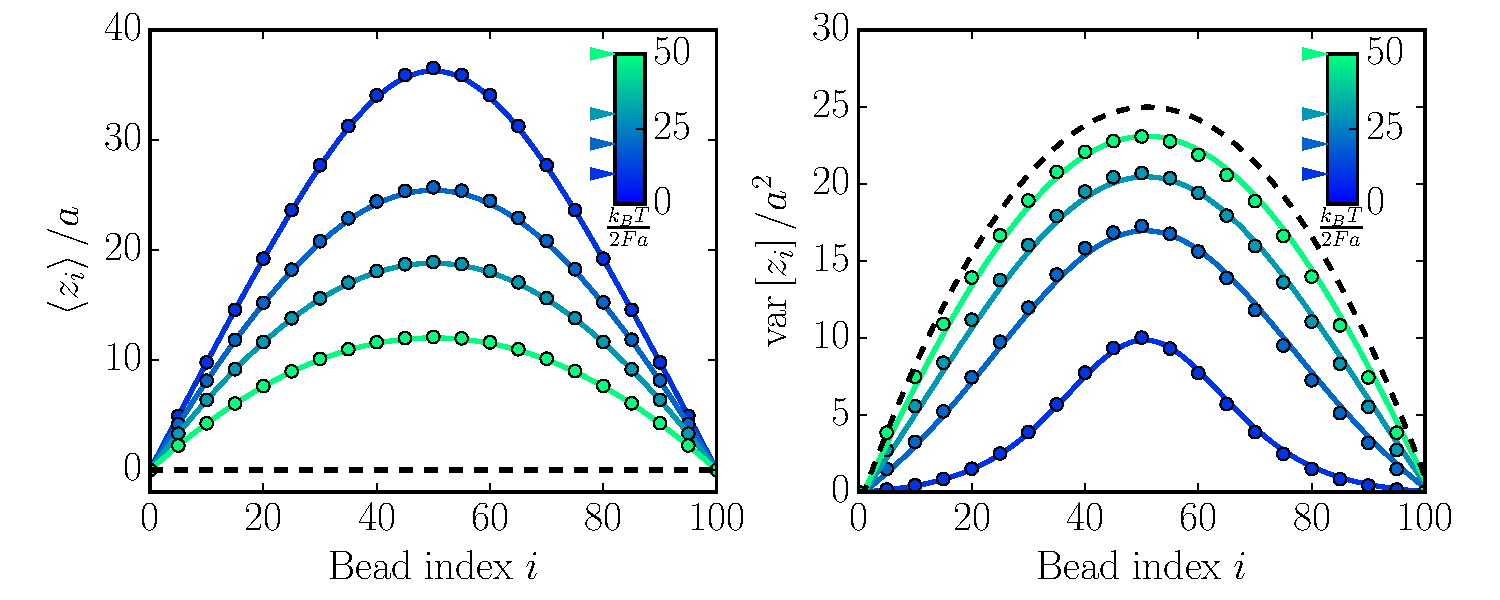
\includegraphics[width=1.0\linewidth]{meanVar}
    \caption{Mean and variance of the 1D polymer loop.}
    \label{fig:meanVar}
\end{figure}

In this section, we have shown that the combination of the Fermi--Dirac statistics following from the grand canonical treatment of the system together with the Brownian bridge condition for random walks provides an excellent approximation for the statistics of the pinned polymer loop. In the next section, for the sake of completeness we show how the same problem can be addressed exactly in the canonical ensemble picture.

\subsection{Fermion integer number partition theory}
\label{sec:numberPartition}

Although the above approach accurately estimates the mean and variance of equilibrium position of every bead, it is an approximated theory. Exact analytic solution is possible in this particular model and helps to establish links to the number theory and theory of ASEP. First we change the basis of the fermionic system from its microscopic configurations $\left\{Z_0,Z_1,\ldots,Z_{L-1}\right\}$ to the total energy of the system. Clearly, the energy can only take values $E_0, E_0+\Delta E, \ldots, E_0 + L^2 \Delta E / 4$ where $E_0$ is the ground state. In this picture, the probability space is a one-dimensional lattice with finite support. Without loss of generality, we set the constant energy $E_0=0$ and $\Delta E=1$. The difficulty of this basis is to determine the degeneracy of the microscopic states which have the same energy $E \in \left\{0,1,\ldots L^2/4\right\}$, referred to as the density of states in statistical mechanics \cite{huang1987statistical} and condensed matter physics \cite{sander2009advanced}. We denote the number of microscopic states with energy $E$ to be $g(E)$; once $g(E)$ is known, the partition function of the system can be formally derived in the canonical ensemble picture
\begin{equation}
\mathcal{Z}\left(T\right) = \sum_{E=0}^{L^2/4} g(E) \, \exp \left(-\frac{E}{k_B T}\right),
\label{eq:par_func}
\end{equation}
and consequently the equilibrium properties of the system can be derived from it. 

Interestingly the problem of finding $g(E)$ can be solved with the help of the closely related problem of integer partition in number theory \cite{andrews1998theory}. 
The connection can be seen in the following way. Consider the system with the energy $E=\sum_{n=1}^{L/2}E_n$, where $E_n$ is the energy of the $n^{\rm{th}}$ particle. Then $g(E)$ is the number of possible ways to partition integer $E$ into the summation of $L/2$ integers with the constraint $0\le E_1\le E_2\cdots\le E_{L/2}\le L/2$.
A very intuitive way to visualize such microscopic configurations is to use the Young diagram \cite{andrews1998theory}. From the number theory \cite{andrews1998theory} we can find the generating function of $g(E)$ (see Appendix X), which turns out to be the Gaussian binomial coefficient:
\begin{equation}
    \Phi (q) := \sum_{E=0}^{L^2/4} g(E) q^E = \left(\begin{array}{c} L \\ L/2 \end{array}\right)_q
\label{eq:generating}
\end{equation}
By comparing Eqs.(\ref{eq:par_func}) and (\ref{eq:generating}) we can find an explicit and exact formula for the partition function of the polymer loop problem:
% \begin{equation}
%     \mathcal{Z}\left(T\right) = \Phi \left(e^{\frac{-\Delta E}{k_B T}}\right) = \frac{\prod_{j=L/2+1}^{L} \sum_{i=0}^{j}e^{-i\Delta E/k_{B}T}}{\prod_{j=1}^{L/2} \sum_{i=0}^{j}e^{-i\Delta E/k_{B}T}}.
% \label{eq:par_func_exact}
% \end{equation}
\begin{equation}
\label{eq:par_func_exact}
    \mathcal{Z}\left(T\right) = \Phi \left(\exp\left(-\frac{\Delta E}{k_B T}\right)\right) 
\end{equation}


By knowing the exact partition function we can calculate the occupation probability of each site, see Appendix \ref{sec:}. {\color{red} can we have a formula here? or it is too big?}. For large $L$ the exact result is almost indistinguishable from our approximate theory based on Brownian bridges approach. However, for sufficiently small $L$ the difference becomes more apparent (see Fig. X in Appendix B). Thus we have demonstrated that the polymer loop model can be related to and solved exactly in terms of the integer number partitioning problem. This, however, is not the last analogy we are going to utilize in this paper.

Here we have to note the connection of the considered problem to the ASEP setup on an interval with reflecting boundaries \cite{}, where an analogous partition function was calculated \cite{}. This demonstrates the equivalence of our model of pinned polymer loop to the ASEP system with reflecting boundaries with exactly one half of the lattice sites occupied by the particles. In the next sections we further exploit this analogy to study the dynamics of the polymer loop model.

\section{Mapping to ASEP}\label{sec:asep}
Above we considered a one-dimensional lattice with $L$ lattice sites filled by $L/2$ particles. So far we were concerned only with the equilibrium properties of the system. However, by noticing the analogy to the ASEP model we can step
beyond equilibrium considerations and study the dynamics of our system. To establish the link of the polymer loop model and the ASEP system we need to understand the relation between polymer dynamics and hopping rules of the ASEP.  A particle occupying a lattice cite corresponds to a monomer of the polymer loop pointing along the direction of force. 
Hopping of a particle on a lattice corresponds to the flipping of two monomers connecting to the same bead and having the opposite orientations with respect to the force field (see illustration in Fig. \ref{fig:asep}). During this flip, the bead has to travel a distance of $\pm2a$. Indeed, just like in the exclusion process, the flip can occur only if there is a ``free'' lattice site. The asymmetry of the flipping results from the force acting on the beads: if, as a result of the flip, the bead moves along the force, it will be energetically more favorable than flipping the bead against the force. We can now formalize such dynamics by using the language of the ASEP model \cite{Derrida1998,Schutz2001}. 
 \begin{figure}[htpb]
     \centering
     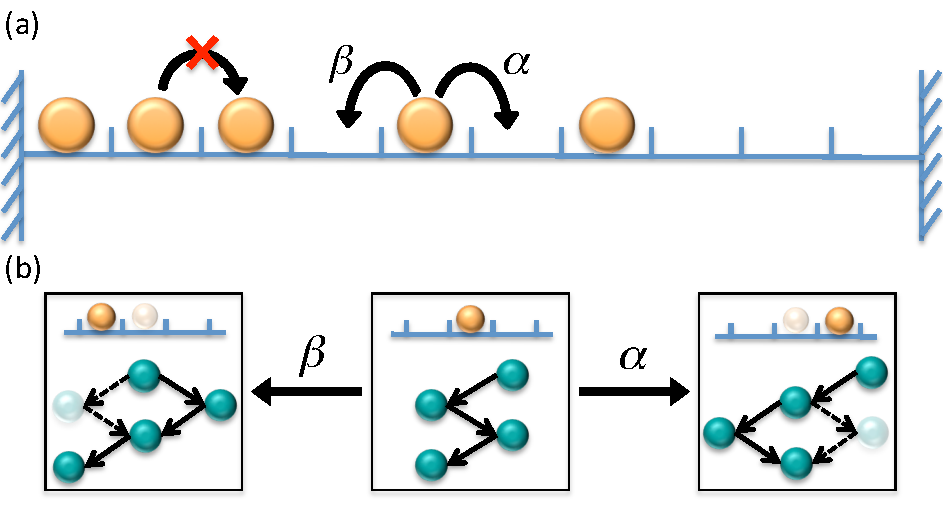
\includegraphics[width=1.0\linewidth]{asep}
     \caption{Illustration of dynamics maps to ASEP.}
     \label{fig:asep}
 \end{figure}
We denote the rate of particle hopping to the right and to the left with $\alpha$ and $\beta$ respectively. For reflecting ASEP, the detailed balance relation holds in equilibrium, so we have {\color{red} do we need this statement? if it only works at equilibr. how can we use it to study dynamics?}
\begin{equation}
    \alpha P_{l} = \beta P_{l+1} \label{eq:db}
\end{equation}
where $P_{l}$ is the probability of a particle to occupy $l^{\rm{th}}$ site. The ratio of rates (and thus of the neighboring occupation probabilities) is proportional to the Boltzmann factor with the energy difference between the two states:
\begin{equation}
    \alpha / \beta = P_{l+1} / P_{l} = \exp{(-\Delta E / k_B T)},  \label{eq:r_divide_l}
\end{equation}
where  $\Delta E = 2Fa$.  The total hopping rate of a particle is determined by the effective temperature of the system: 
\begin{equation}
    \alpha + \beta = r_{\text{total}} \label{eq:l_plus_r}
\end{equation}
Hopping of a particle to the neighboring lattice site corresponds to flipping of two monomers and the displacement of the bead by a distance of $2a$. In the force-free case this flipping happens due to thermal fluctuations. Note that in the strictly one-dimensional setting, the monomers can not continuously turn, there are just initial and final states along or against the field. Therefore, for now we only provide an estimate of the time scale required for making a flip, a time for a bead to freely diffuse a distance $2a$ 
\begin{equation}
    \label{eq:timeScale}
    % D=\frac{4a^2}{2\tau_0}=\frac{k_{B}T}{\gamma}; \quad \tau_0=\frac{2\gamma a^2}{k_{B}T}=r_{\text{total}}^{-1}.
    r_{\text{total}}^{-1} = \tau_0 \propto \frac{(2a)^2}{2D} = \frac{2\gamma a^2}{k_{B}T}.
\end{equation}
where we used the diffusion constant of the bead given by Einstein relation $D=k_{B}T/\gamma$, where $\gamma$ is the friction coefficient. Importantly, later we will be able to determine the proper calibration of this hopping rate by benchmarking our results with the Rouse theory (see below). 
% $\gamma=6\pi R\eta$, $\eta$ is viscosity of the surrounding fluid, and $R$ is the radius of the bead. 
Finally, from Eqs.(\ref{eq:r_divide_l},\ref{eq:l_plus_r}) we obtain for the left and right hopping rates:
\begin{subequations}
    \label{eq:l_and_r}
    \begin{eqnarray}
        \alpha  =   \frac{r_{\text{total}}\exp{(-2Fa / k_B T)}}{1+\exp{(-2Fa / k_B T)}} \\
        \beta  =  \frac{r_{\text{total}}}{1+\exp{(-2Fa / k_B T)}}
    \end{eqnarray}
\end{subequations}
Next we need to specify the boundary conditions and if there any additional constraints on the number of particles. The pinned polymer loop corresponds to exactly $L/2$ particles hopping on $L$
lattice sites with reflecting boundary conditions. The mapping can be generalized to other cases, for example,
an un-pinned polymer loop corresponds to $L/2$ particles on $L$ lattice sites with
periodic boundaries, free polymer chain corresponds to an open lattice of length $L$ filled by
arbitrary (but not larger than $L$) number of particles. 

ASEP is one of the fundamental models of non-equilibrium statistical physics with a wealth of important analytical results, see \cite{} for a review. However, not so many works are dealing with the particular case of reflective boundary conditions. One important contribution is due to Schuetz \cite{} where the partition function identical to Eq.(\ref{eq:par_func_exact}) was derived. Here our main motivation is to get an insight on the dynamics of the system. 

\section{Exact solution of ASEP dynamics}
We show that the exact analytical solution of the ASEP model with reflecting boundaries can be obtained by using the Bethe-ansatz. To demonstrate the logic of derivation we first consider the simplest case of 2 particles on $L$-size lattice and then generalize it to arbitrary $N\leq L-1$.
%To illustrate the procedure of solving the dynamics, we firstly present here the simple example of two particles system. The generalization to $N$ particles case is straight forward and details will be discussed in the Appendix.

Let us denote $P(x_1, x_2; t)$ the time dependent probability of finding the first and the second particle at coordinates $(x_1, x_2)$ respectively, where $x_1, x_2$ are integers. One can write down the master equation and boundary conditions which define the dynamics of the system, see appendix B. To solve for the dynamics, we first use the standard variable separation ansatz $P(x_1, x_2; t) = \sum_k { \Psi_k(x_1, x_2) e^{\Lambda_k t}}$. Now the task is to find $\Psi_k$ and the corresponding eigenvalues $\Lambda_k$. The main idea of the generalized Bethe-ansatz is to use the general form of single-particle eigenfunctions as building blocks to construct $\Psi_k$ (in contrast to plane waves in the standard Bethe-ansatz previously employed in the ASEP model with periodic boundaries \cite{}). The ansatz we use here can be written as follows:
\begin{equation}
    \label{eq:ansatzTwo}
    \Psi(x_1, x_2) = \psi_1(x_1)\psi_2(x_2) + \tilde{\psi}_2(x_1)\tilde{\psi}_1(x_2)
\end{equation}
where $\psi_n, \tilde{\psi}_n, n=1,2$ are functions drawn from the following general form of the single-particle eigenfunctions:
\begin{subequations}
    \label{eq:eigenModes}
\begin{eqnarray}
    \label{eq:stationaryEigenMode}
    &\psi_s(x)  =  A\left(\frac{\alpha}{\beta}\right)^x \\
    \label{eq:nonstationaryEigenModes}
    &\psi_{ns}(x)  =  \left(\frac{\alpha}{\beta}\right)^{\frac{x}{2}}
    \left(A_+ e^{ipx} +  A_-e^{-ipx}\right) 
\end{eqnarray}
\end{subequations}
Here, $A,~A_+,~A_-$ are amplitudes that will be fixed by the boundary conditions and normalization, $p$ is the wave vector of the excited eigenmodes (in the case of a single particle $p=\frac{k\pi}{L}$, $k=1,2,...,L-1$).

Following the single-particle terminology we will distinguish two classes of eigenfunctions: $\psi_s(x)$ given by Eq. \eqref{eq:stationaryEigenMode} to be referred to as stationary and $\psi_{ns}(x)$, Eq.(\ref{eq:nonstationaryEigenModes}) non-stationary eigenfucntions. Now $\psi_n(x)$ with $n=1,2$ can be chosen from either class. Functions $\psi_n$ and  $\tilde{\psi}_n$  with and without tilde with the same subscript belong to the same class and have the same wave vector (in the non-stationary case) but may differ by the amplitudes. %These amplitudes can be determined from the conditions on $\Psi(x_1, x_2)$ to satisfy the reflecting boundaries and exclusive conditions, Eqs. \eqref{eq:boundaries-two-particles} and \eqref{eq:exclusionCondition} respectively.  

There are three types of $\Psi(x_1, x_2)$ depending on the combination of $\psi_n(x)$ entering its definition Eq.(\ref{eq:ansatzTwo}): both stationary, both non-stationary, and the mixed type with one stationary and the other one non-stationary. The first case leads to the stationary mode of the two particles system with eigenvalue $\Lambda_0 = 0$ and $\Psi_0(x_1, x_2) = A \left(\frac{\alpha}{\beta}\right)^{x_1+x_2}$. $A$ is a constant that can be fixed by normalization (for details see Appendix ?? for the general case of $N$ particles).

The second type (both $\psi_n(x)$ are non-stationary) of $\Psi(x_1, x_2)$ when substituted in the boundary and exclusion conditions leads to the following system of Bethe equations \cite{} (see Appendix ?? for details):
\begin{subequations}
    \label{eq:betheEqTwo2}
    \begin{eqnarray}
        e^{i2p_1L} & = & \frac{a(p_1, p_2)}{a(p_2, p_1)} 
        \frac{a(p_2, -p_1)}{a(-p_1, p_2)}\\
        e^{i2p_2L} & = & \frac{a(p_2, p_1)}{a(p_1, p_2)} 
        \frac{a(p_1, -p_2)}{a(-p_2, p_1)}
    \end{eqnarray}
\end{subequations}
where $a(p, p^\prime) = \sqrt{\alpha\beta}e^{i(p+p^\prime)}-(\alpha+\beta)e^{ip}+\sqrt{\alpha\beta}$. 
The corresponding eigenvalues can be calculated by $\Lambda = \sum_{n=1}^2 -(\alpha+\beta)+2\sqrt{\alpha\beta}\cos(p_n)$. Notice that by solving Eq. \eqref{eq:betheEqTwo2} we can get multiple pairs of roots because it is a set of nonlinear equations. 
{\bf Let me try to rephrase in details... Too detailed. Here I suggest just to state how many eigenvalues we will get from this part.} 
    %The roots pair $(p_1, p_2)$ with different values can lead to different eigenvalues, e.g. it is possible that $(p_1, p_2) = (\pi/2, \pi/3)$ and $(p_1, p_2) = (\pi/4, 2\pi/3)$ are both the solution of Eq. \eqref{eq:betheEqTwo2}, and the eigenvalue $\Lambda$ obtained from these two roots are different. So we will get more than one eigenvalues here. However, we have to discard the roots such like $(p_1, p_2) = (\pi, \pi/3)$ or $(p_1, p_2) = (\pi/2, \pi)$, basically the roots either $p_1$ or $p_2$ or even both equal to $k\pi$. Because $p_1 = \pi$ means that $\psi_1$ is actually in stationary mode. (Notice the index $k$ of single particle non-stationary eigenfunction is from $1$ to $L-1$, there are $L$ different eigenvalues in total.) In this case, the ansatz of $\Psi$ is no longer type two (two non-stationary). It should belong to either type one or type three. And the expression for different type $\Psi$ as well as eigenvalues are not compatible to each other. That is why we have to discuss three different cases separately. 

The third type of $\Psi(x_1, x_2)$ (mixed) can be solved similarly to the second type. Interestingly, the resulting Bethe equation is very simple (we assumed that $\psi_1(x)$ is stationary):
\begin{equation}
    \label{eq:betheEqTwo1}
    e^{i2p_2L} = 1
\end{equation}
by solving which we get $p_2 = \frac{k\pi}{L}$ and the corresponding eigenvalues $\Lambda_k = -(\alpha+\beta)+2\sqrt{\alpha\beta}\cos(p_2)$ (see Appendix ??). These eigenvalues are exactly the same as for the single particle hopping on a lattice of size $L$ with reflecting boundaries. 

Thus we have shown how to employ the generalized Bethe-ansatz on the example of two particles. As the outcome we get three types of eigenstates: stationary, non-stationary with Bethe equations, and the mixed state leading to one-particle solution. We now show how to generalize this result to arbitrary $N$ and discuss the general properties of the solution.  %Actually, we can show later that the set of eigenvalues of $N+1$ particles system always contain the set of eigenvalues of $N$ particles system given that they have the same lattice sites $L$ and $N<L/2$. For $N>L/2$, one can simply apply the particle-hole duality and obtain that the spectrum of $N$ particles system is the same as the $L-N$ particles system.

%Unlike the second type of $\Psi(x_1, x_2)$ that the Bethe Equations have to be solved numerically in general, the expression of eigenvalues and eigenfunctions can be obtained analytically for the third type which are summarized as following:
%\begin{subequations}
%    \label{eq:eigenTwo}
%    \begin{equation}
%        \label{eq:eigenvaluesTwo}
%        \Lambda_k  = -(\alpha+\beta) + 2\sqrt{\alpha\beta}\cos(\frac{k\pi}{L});
%        k=1,2,\dots, L-1
%    \end{equation}
%    \begin{equation}
%        \label{eq:eigenvectorsTwo}
%        \Psi_k(x_1, x_2)  =  A\left[ \frac{\alpha}{\beta}
%            \left(\frac{\alpha}{\beta}
%            \right)^{x_1}\phi_k(x_2)+\left(\frac{\alpha}{\beta}\right)^{x_2}
%            \phi_k(x_1) \right]
%    \end{equation}
%\end{subequations}
%Here $\phi_k(x)$ is exactly single particle non-stationary eigenfunction and
%$A$ is a constant normalization coefficient. Fortunately, numerical evidence shows that the most interesting eigenvalue, i.e., the largest non-zero eigenvalue which corresponds to the slowest relaxation mode, is contained in this analytical set. See appendix for more details.

%Now let us sketch the generalization from two particls to $N$ particles system. The details are shown in appendix. 
The Bethe-ansatz for the $N$ particle solution can be written as
\begin{equation}
    \label{eq:ansatzN}
    \begin{aligned}
        \Psi(x_1, x_2, \cdots, x_N) = \sum_{\sigma\in \mathcal{S}_N}
        \prod_{n=1}^N \psi_n^{\sigma}(x_{\sigma(n)})
    \end{aligned}
\end{equation}
where $\mathcal{S}_N$ is the group of permutations of $N$ elements and $\psi_n^{\sigma}$ is the $n^{\text{th}}$ class of eigenfunction drawn from Eq.  \eqref{eq:eigenModes}, either stationary or non-stationary. The subscript $n$ means all functions in the $n^{\text{th}}$ class share the same $p_n$, the superscript $\sigma$ means the amplitude coefficients $A_n^{\sigma}$ or $A_{n\pm}^{\sigma}$ are not the same for different permutations.

The stationary solution can be obtained by constructing $\Psi$ only from stationary $\psi_s$, after normalization (see appendix A), we get: 
\begin{equation}
    \label{eq:stationarySolutionN}
    P^e(x_1, x_2, \cdots, x_N) = q^{-\frac{N(N+1)}{2}}
    \binom{L}{N}_q^{-1}\prod_{j=1}^N{q^{x_j}}
\end{equation}
here $q:=\frac{\alpha}{\beta}$. The prefactor here is identical to the partition function from Sec.II C and the results of Ref.\cite{} where a method based on $U_q(SU(2))$ quantum group was utilized.

If all building blocks of $\Psi$ are non-stationary, we arrive at the following Bethe equations:
\begin{equation}
    \label{eq:betheEqN}
    e^{i2p_nL}  =  \prod_{m\neq n}^N\frac{a(p_n, p_m)}{a(p_m, p_n)} 
    \frac{a(p_m, -p_n)}{a(-p_n, p_m)}
\end{equation}
We can resolve them for $p_n$ and find the corresponding eigenvalues $\Lambda=\sum_{n=1}^N -(\alpha+\beta) + 2\sqrt{\alpha\beta}\cos(p_n)$. 

Finally let us consider the mixed case with $N_s$ stationary building blocks in $\Psi$ and $N-N_s$ non-stationary, where $0<N_s<N$. One can show that the resulting Bethe equations are identical to the case of $N-N_s$ particles system when all building blocks are non-stationary. Moreover, the corresponding eigenvalues are $\Lambda = \sum_{n=1}^{N-N_s} -(\alpha+\beta)+2\sqrt{\alpha\beta}\cos(p_n)$. Therefore we can conclude that the set of eigenvalues of $N$ particle system always contains the set of eigenvalues of $N-N_s$ system given that $N<L/2$ (for $N>L/2$ we can instead look at vacancies and apply similar considerations). This is a generalization of the result of the two-particle system.

The central technical difficulty is to solve the Bethe equations to get the wave vectors and the corresponding set of the eigenvalues. It is a non-trivial task to show that the eigenstates obtained through the Bethe-ansatz approach indeed form a complete set, see for example \cite{}. We, so far, used the numerical solution of Bethe equations and compared thus obtained results for eigenvalues with the direct diagonalization of the transition matrix in the master equation, see Fig. ??. In the figure we also show that the eigenvalues of the system with a smaller number of particles are always contained in the case of the system with larger $N$. Importantly, the subset of eigenvalues corresponding to the single particle solution can always be calculated explicitly: 
%we remark that the Bethe Equations have to be solved numerically in most cases. However, there is a small set of non-stationary eigenvalues and eigenvectors we can obtain analytically, which correspond to the case with just one excitation mode. The results are summarized as following:  
% \begin{subequations}
%     \label{eq:eigenN}
    \begin{equation}
        \label{eq:partEigenvaluesN}
        \Lambda_k   = -(\alpha+\beta) + 2\sqrt{\alpha\beta}\cos(\frac{k\pi}{L}); 
        k=1,2,\dots, L-1  
    \end{equation}
  %  \begin{equation}
%        \label{eq:eigenvectorsN}
%        \Psi_k(x_1, x_2, \cdots, x_N)  =  A \sum_{n=1}^N
%        \left(\frac{\alpha}{\beta}\right)^{n-1} \phi_k(x_n)\prod_{m\neq n} 
%         \left(\frac{\alpha}{\beta}\right)^{x_m}
%    \end{equation}
% \end{subequations}
\begin{figure}[htpb]
    \centering
    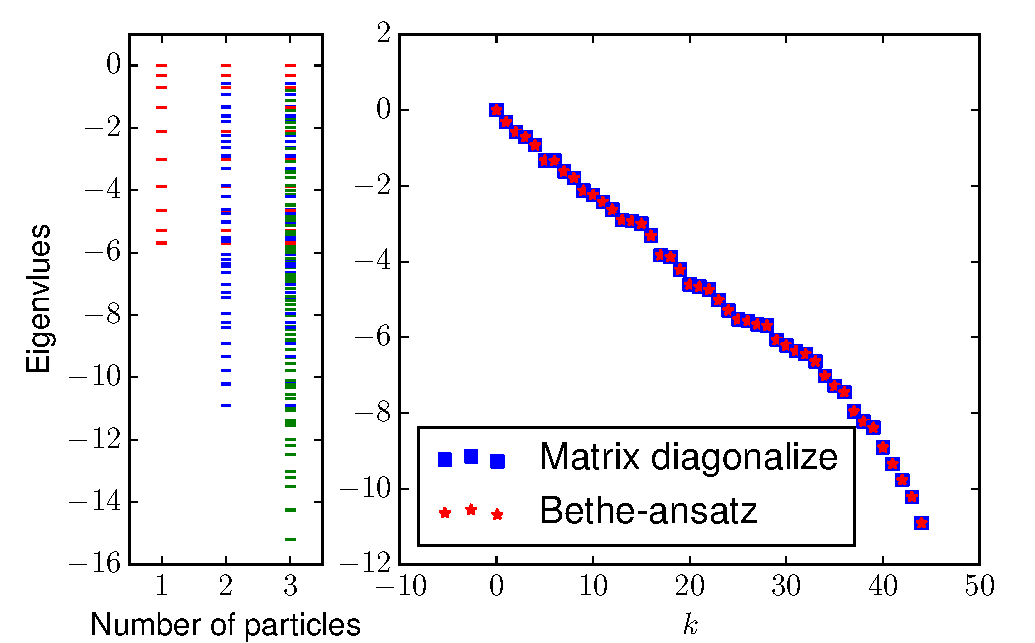
\includegraphics[width=1.0\linewidth]{spectrum}
    \caption{eigenvalue obtained from directly diagonalizing the transition matrix and comparison with the results from Bethe-ansatz.}
    \label{fig:spectrum}
\end{figure}


Numerical evidences shows that the single particle solution provides the largest non-zero eigenvalue ($k=1$) which does not depend on the particles number $N$, thus giving us a direct estimate of the longest relaxation time in the system.  

%With the exact solution of ASEP in hand, we now extract a physical quantity that interested us, i.e. relaxation time. It is related to the largest non-zero eigenvalue $\Lambda_1$ of the system. Here we pick the largest one from the analytical set of eigenvalues and postulate that it is the largest non-zero eigenvalue. Namely, $\Lambda_1 = -(\alpha+\beta) + 2\sqrt{\alpha\beta}\cos(\frac{\pi}{L})$. This statement is difficult to prove rigorously given that the Bethe Equations have to be solved numerically in most cases. However, numerical results from both direct diagonalizing the transition matrix and Kinetic Monte-Carlo simulation of the ASEP process show that the statement is indeed true. See Fig. \ref{fig:relaxation1D} and Fig. Sx. Accordingly, the explicit form of relaxation time of the system can be written as 

\begin{equation}
    \label{eq:relaxationTime}
    \tau = -\frac{1}{\Lambda_1} = \frac{1}{\alpha+\beta-2\sqrt{\alpha\beta}\cos(\frac{\pi}{L})}
\end{equation}
Notice that an inexact result is also obtained in \cite{}, and is different from our exact result Eq. \eqref{eq:relaxationTime} only by a factor $\sqrt{\alpha\beta}$. We can now consider several important limiting cases of this expression, when $L$ is large we can expand the cosine term and get $\tau = 1/\left((\sqrt{\alpha}-\sqrt{\beta})^2 + \sqrt{\alpha\beta}\pi^2/L^2\right)\approx 1/(\sqrt{\alpha}-\sqrt{\beta})^2$. In the case of zero force $\alpha=\beta$, we arrive at $\tau=L^2/\sqrt{\alpha\beta}\pi^2$. This relaxation time can be independently obtained from the Rouse theory, which considers the polymer loop as a chain of beads connected by ideal springs. The classical model \cite{} needs to be modified to accommodate the constraint of the pinned loop (see Appendix ?? for derivation) but gives the same standard Rouse time. Importantly we can now use the Rouse time to fix the hopping rate in our one-dimensional polymer loop model:
\begin{equation}
    \label{eq:timeScale_corrected}
    % D=\frac{4a^2}{2\tau_0}=\frac{k_{B}T}{\gamma}; \quad \tau_0=\frac{2\gamma a^2}{k_{B}T}=r_{\text{total}}^{-1}.
    r_{\text{total}}^{-1} = \frac{\gamma a^2}{2k_{B}T}.
\end{equation}
 To further test analytical predictions of this section we numerically investigated the process of relaxation in the one-dimensional pinned polymer loop by kinetic Monte-Carlo simulations. To quantify the relaxation times we looked at the time correlation function of the diameter of the polymer defined by $r_d = r_{L/2} - r_0$. For large times it shows an exponential decay, see inset in Fig.5. This allows us to determine the characteristic time of decaying correlations and associate it with the relaxation time of the loop. We see that the relaxation times plotted as a function of the external force match perfectly the analytical prediction given by the Bethe-ansatz solution, Eq.(\ref{eq:relaxationTime}), see Fig 5.


\begin{figure}[htpb]
   \centering
   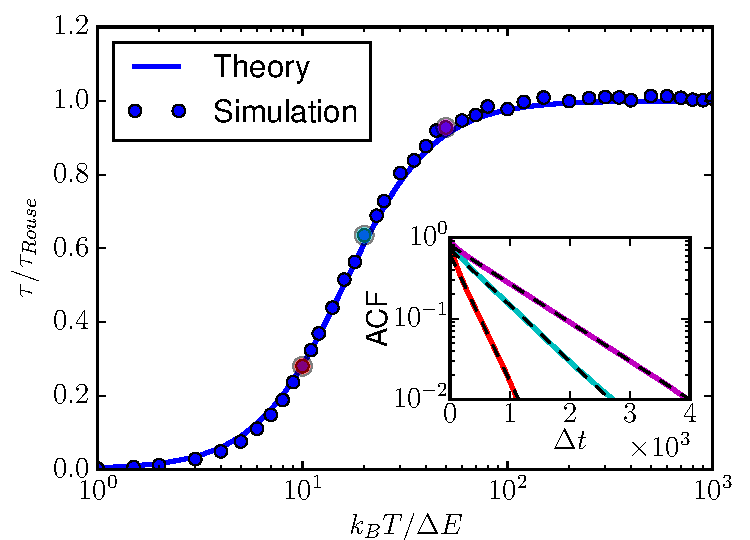
\includegraphics[width=1.0\linewidth]{relaxation1D}
   \caption{relaxation time of ASEP for different force setting.}
   \label{fig:relaxation1D}
\end{figure}



% To find the solution of the ASEP model we use the generalized Bethe-ansatz in which the $N$-particle density of particles is sought in the following form:
%
% {\bf Wenwen, please add brief version of the derivation here. I add a short list to guide what else to include}
%
% Give the form of the ansatz, give the boundary condition and non-crossing condition. Provide the answer for a single particle PDF. All details, like checking the boundary conditions and derivation of 1 particle pdf should go to Appendix A. 
%
% Provide a statement that the stationary solution is the same as from number theory.
%
% Give formula for the longest relaxation time. Discuss its force, number of particles, and temperature dependence. 
%
% Compare it to Schutz result.
%
% Make a statement about the limit of $F\leftarrow 0$ and mention that it can be recovered via the Rouse model approximation (we shouldn't give derivation in this paper, you may refer to to be published (which is your thesis)).
%


Thus, starting from the biological problem of chromosome alignment we could unfold a very rich sequence of analogies and obtained the whole set of analytical results relevant for both polymer and non-equilibrium particle systems. To make the loop complete, now in the sense of paper structure, we would like to demonstrate how the above analytical results can be put to work in a more applied setting.


\section{Relaxation dynamics of a 3D polymer loop}
Previously we argued that the stationary solution for the pinned polymer loop could be used to quantify the chromosome separation during meiosis in fission yeast \cite{}. However a very reasonable question is if the stationary state could be achieved on biologically relevant time scales. To answer this question we suggest to look at the relaxation dynamics of the pinned polymer loop as a function of parameters of the problem and in particular the applied external force. We performed extensive three-dimensional Brownian dynamics simulations of the relaxation process of the 3D polymer loop. By calculating the autocorrelation function of $z$ component of diameter vector, we could extract the longest relaxation time of the polymer loop and plot it as a function of the applied force (see Fig.X). The relaxation times show the behavior very similar to our analytical prediction for the one-dimensional problem. We hypothesized that the functional form of Eq.(\ref{eq:relaxationTime}) could be used to describe the results of the 3D simulations. Importantly, we know that the relaxation time in the limit of $F\rightarrow 0$ can be calculated from the Rouse-theory analytically (see Appendix ??).  The result is identical to the 1D regime with an additional prefactor of 1/3 which arises due to the difference between 1D and 3D settings. We now can use this prefactor in the analytical formula Eq. \eqref{eq:relaxationTime} and plot it together with simulation results. Analytical (rescaled on the basis of the Rouse-theory) prediction matches the simulations very accurately. Note that there was no fitting involved when comparing theory and numerical data. Certainly the achieved agreement of theory and data is a somewhat semi-empirical result, as we did not provide any three-dimensional theory except for the Rouse limit $F\rightarrow 0$. Nevertheless the one-dimensional model allows us to understand exactly the mechanisms responsible for the relaxation process in the system. It also makes it plausible to suggest that our results can be rigorously extended to higher dimensions.
\begin{figure}[htpb]
    \centering
    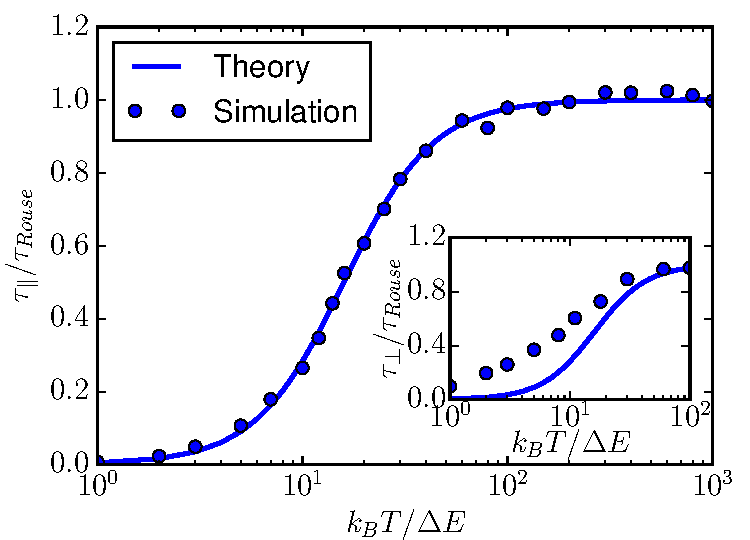
\includegraphics[width=1.0\linewidth]{relaxation3D}
    \caption{relaxation time of 3D pinned polymer.}
    \label{fig:relaxation3D}
\end{figure}
 
\section{Conclusions}
We demonstrated that the problem of the pinned 1D polymer loop in the external force field can be mapped to a system of particles hopping on lattice sites (ASEP). While the polymer problem can be asymptotically solved via the Brownian bridge formalism, in the ASEP formulation it has an exact solution. ASEP advances our understanding of the system to the dynamic regime. The key technique for the ASEP model solution is the generalized Bethe-ansatz, adding up to the Fermi-Dirac statistic as yet another unexpected appearance of quantum-mechanics tools in an original biophysical problem. Finally we could use those results to explain the force dependence of the relaxation times observed in 3D Brownian dynamics simulations.

In addition to the network of relations between different models and approaches we would like to mention yet another connection arising from the ASEP model. It is well known that ASEP models are often used as discrete counterparts of the single file diffusion process []. In single file diffusion, particles are considered to be confined to a narrow one-dimensional channel which does not allow the particles to overcome each other. As the name implies, individual particles move by normal diffusion. It can be shown that the solution for the ASEP with reflecting boundaries can be used to described the single file diffusion on a confined interval in the external force field. The crucial difference is that in case of single file diffusion particles are allowed to move continuously instead of lattice hopping in ASEP. Interestingly, a proper generalized Bethe-ansatz can be used to solve for the dynamics in this problem as well \cite{}. 

The mapping from polymer to particles is not restricted to the case of pinned polymer loop. Other situations can be investigated with the same mapping, which leads to ASEP model with different boundaries and particle numbers. Moreover, the polymer dynamics beyond 1D is also possible to
model by multi-species ASEP model \cite{}. We believe that by showing the unity of such apparently different systems we pave the way to their better understanding and hopefully to further new results.
\begin{acknowledgments}
We would like to acknowledge stimulating discussions with S. Majumdar and E. Frey.\end{acknowledgments}


\appendix


\section{Stationary statistics}
\label{sec:stationary_statistics}
We mention in the main text three different ways to get the stationary statistics. We will compare and benchmark the results here.

The first methods is an approximation method use \emph{grand canonical ensemble} and the technique of Brownian bridge. The approach is sketched in the main text, we will show here the stationary statistics of the pinned 1D polymer, i.e., mean and variance of monomers position.

According to Eq. \eqref{eq:z2x} and Eq. \eqref{eq:zmean}, the mean position of the 1D polymer monomer can be written as 
\begin{equation}
    \label{eq:polymerMeanPos}
    \left< z_i \right> = a \left( 2 \sum_{j=0}^i \mathbb{E}\left[Z_j\right] - i \right)
\end{equation}
The variance of monomer position is given by Eq. \eqref{eq:zvar} and Eq. \eqref{eq:bridgeVar}. Plug in Eq. \eqref{eq:discrete_prob} and convert the summation to integral when $T\gg 1$, we obtain
\begin{subequations}
    \label{eq:meanVarPolymerPos}
    \begin{eqnarray}
        \left< z_i \right> = 2 a \tilde{T} \ln\left[ \frac{1+\exp\left(\frac{L}{2\tilde{T}}\right)}{\exp\left(\frac{i}{2\tilde{T}}\right) + \exp\left(\frac{L-i}{2\tilde{T}}\right)} \right] \\
        \text{var}\left[z_i\right] = 2 a^2 \tilde{T} \frac{ \sinh\left( \frac{L-i}{2\tilde{T}}\right) \sinh\left( \frac{i}{2\tilde{T}}\right)} {\sinh\left( \frac{L}{2\tilde{T}}\right) \cosh^2\left( \frac{L-2i}{4\tilde{T}}\right)}
    \end{eqnarray}
\end{subequations}
where $\tilde{T} = k_B T / 2Fa$. 

The second method use \emph{canonical ensemble} with number partition theory and the third method use Bethe-ansatz obtaining the stationary state of ASEP are both exact solution. We will show the exact partition function obtained from these two methods are equivalent and then compare the exact result of density profile to the \emph{Fermi-Dirac} approximation of the first method.

The exact term of partition function from method two is already listed in Eq. \eqref{eq:par_func_exact}. So let us derive here the exact partition function using method three.
According to the rules of our generalised Bethe-ansatz, the $N$ particles stationary solution of the ASEP system can be constructed as
\begin{equation}
    \label{eq:stationaryN}
    P^e(x_1, x_2, \cdots, x_N) = \Psi_0(x_1, x_2, \cdots, x_N) =  A
    \prod_{j=1}^N\left(\frac{\alpha}{\beta}\right)^{x_j}
\end{equation}

One can plug it in the master equation check that the corresponding eigenvalue $\Lambda_0= 0$, and also verify the exclusive condition as well as the reflecting boundaries are both fulfilled.
Remember that $\alpha/\beta = \exp\left( - \Delta E / k_B T\right)$, one can see clearly the connection between Eq. \ref{eq:stationaryN} and the partition function after do a variable transfer and rewrite it as 
\begin{equation}
    \label{eq:stationaryNRewrite}
    P^e(x_1, x_2, \cdots, x_N) = A \exp\left( -\frac{\Delta E}{k_B T} E\right)
\end{equation}
where $E:=\sum_j{x_j}-E_0$ with $E_0 = 1 + 2 + \cdots + N = \frac{N(N+1)}{2}$. So $E$ is a integer in the range of $0, 1, \cdots, N(L-N)$. One immediately recognize the partition function is related to the normalization prefactor $A$ as following:
\begin{equation}
    \label{eq:partitionFuncBethe}
    \mathcal{Z}(T) = A^{-1} = \sum_{x_1 < x_2 < \cdots < x_N} q^{\sum_j{x_j}}
    = q^{E_0}\sum_{E=0}^{N(L-N)}g(E)q^E
\end{equation}
And $g(E)$ is exact the number of partitions of positive integer $E$ to $N$ parts with each of size at most $L-N$. Further more, we can also identify the Gaussian binomial coefficients
\begin{equation}
    \label{eq:degeneracy}
    \sum_{E=0}^{N(L-N)}g(E)q^E = \binom{L}{N}_q = \frac{[L]_q!}{[L-N]_q![N]_q!}
\end{equation}
where $[N]_q = 1 + q + q^2 + \cdots + q^{N-1}$ is called a $q$ number. So we finally arrive at Eq. \eqref{eq:stationarySolutionN}. Meanwhile, by setting $E_0 = 0$ and $N=L/2$ as we did in section \ref{sec:numberPartition}, we obtain exactly the same partition function as Eq. \eqref{eq:par_func_exact}. We emphasize here that both methods give us correct exact stationary statistics. However, use the Bethe-ansatz method, one can step further into the dynamics. 

With the stationary $N$ particle distribution Eq. \eqref{eq:stationarySolutionN}, we can readily calculate the equilibrium distribution of any tagged particle. Denote he distribution of the $n$th particle $p_n(x)$, we have
\begin{equation}
    \begin{aligned}
        \label{eq:pdfTaggedParticle}
        p_n(x) = & \sum_{0<x_1<\cdots<x_{n-1}\le x-1}P^e(x_1, x_2, \cdots, x_N) \\
        &\times \sum_{x<x_{n+1}<\cdots<x_{N}\le L}P^e(x_1, x_2, \cdots, x_N) \\
        = & \left. q^{(N+1-n)(x-n)} \binom{x-1}{n-1}_q\binom{L-x}{N-n}_q 
            \middle/  \binom{L}{N}_q \right.
    \end{aligned}
\end{equation}
Finally, the equilibrium density profile, which is the exact counterpart of Fermi-Dirac distribution Eq. \eqref{eq:discrete_prob}, can be obtain by summing up $p_n(x)$
\begin{equation}
    \label{eq:densityProfile}
    \rho(x) = \sum_{n=1}^N p_n(x) 
\end{equation}
The exact result is shown in Fig. \ref{fig:densityProfile} and compared with the density profile we get from the Fermi-Dirac approximation. 
\begin{figure}[htpb]
    \centering
    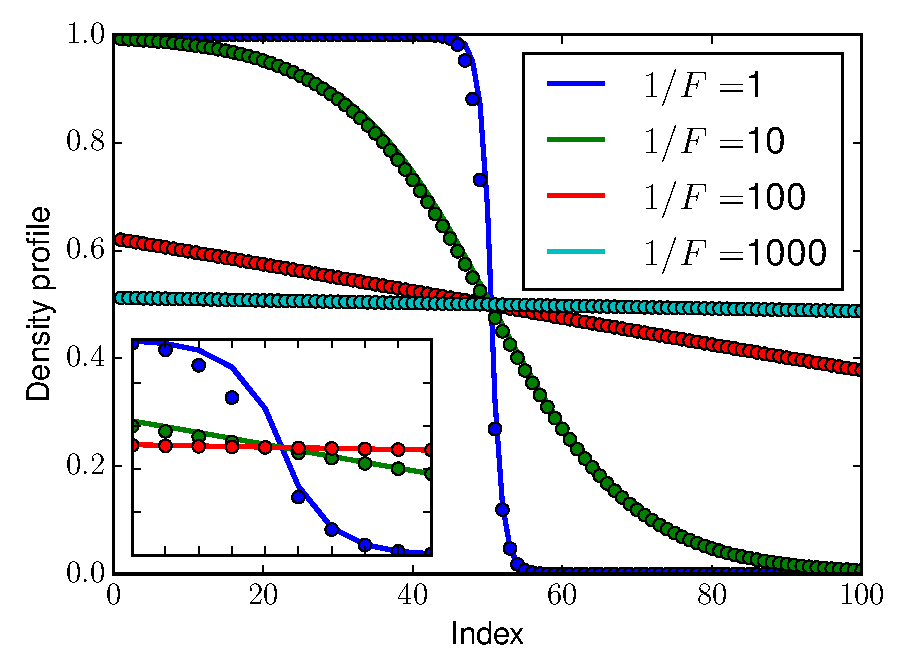
\includegraphics[width=1.0\linewidth]{densityProfile}
    \caption{density profile}
    \label{fig:densityProfile}
\end{figure}


\section{Derivation of the Bethe Equations}
\label{sec:derivation_of_bethe_equations}
To show the derivation of the Bethe Equations, we first show it in the simple two particles case and then generalise to $N$ particles case.

We start by writing down the master equation for the two-particle density assuming both of the particles are neither sitting on the boundary sites nor sitting on the neighboring sites:
\begin{equation}
    \begin{aligned}
    \label{eq:masterEqTwo}
    \frac{d P(x_1, x_2; t)}{dt} = & \alpha P(x_1-1,x_2;t) + \beta P(x_1+1,x_2;t) \\ 
    & + \alpha P(x_1, x_2-1; t) + \beta P(x_1, x_2+1; t)  \\ 
    & - 2(\alpha+\beta)P(x_1, x_2; t)
    \end{aligned}
\end{equation}
where $P(x_1, x_2; t)$ is time dependent probability of finding the first and the second particle  at coordinates $(x_1, x_2)$ respectively. The master equation \ref{eq:masterEqTwo} should be supplemented with reflecting boundary conditions \cite{} 
\begin{subequations}
    \label{eq:boundaries-two-particles}
    \begin{eqnarray}
        \alpha P(0,x_2;t) = \beta P(1, x_2;t) \\
        \alpha P(x_1, L;t) = \beta P(x_1, L+1;t)
    \end{eqnarray}
\end{subequations}
and with the exclusion condition (two particles can not occupy the same lattice cite) \cite{}: %On the other hand, the particle can not pass each other because the exclusive definition. Similarly, one can write down the special master equation when two particles are sitting at the neighboring sites and derive the constraint of exclusion as another boundary condition written as 
\begin{equation}
    \label{eq:exclusionCondition}
    \alpha \Psi(x, x) + \beta \Psi(x+1, x+1) = (\alpha + \beta) \Psi(x, x+1),
\end{equation}
where $x$ is a shorthand notation for $x_1=x_2=x$ and the above equation \eqref{eq:exclusionCondition} must be valid over all lattice cites.
Master Eq. \eqref{eq:masterEqTwo} together with boundary conditions Eqs. \eqref{eq:boundaries-two-particles} and \eqref{eq:exclusionCondition} define the dynamics of the two particles system. Now let us take the ansatz Eq. \eqref{eq:ansatzTwo} and consider two different types of non-stationary eigenmode separately. 

Let us firstly consider the two particles non-stationary eigenmode that two classes of building functions are both non-stationary. Plug the ansatz Eq. \eqref{eq:ansatzTwo} in the reflecting boundaries Eq. \eqref{eq:boundaries-two-particles}, we get
\begin{subequations}
    \label{eq:scatterFactorBoundary2}
    \begin{eqnarray}
        \frac{A_{1+}}{A_{1-}} & = & -\frac{\alpha-\sqrt{\alpha\beta}
                e^{-ip_1}}{\alpha-\sqrt{\alpha\beta} e^{ip_1}}  \\
        \frac{\tilde{A}_{1+}}{\tilde{A}_{1-}} & = & 
        -\frac{\left(\alpha-\sqrt{\alpha\beta} e^{-ip_1}\right) e^{-ip_1L}}
        {\left(\alpha-\sqrt{\alpha\beta} e^{ip_1}\right) e^{ip_1L}}  \\
        \frac{\tilde{A}_{2+}}{\tilde{A}_{2-}} & = & -\frac{\alpha -
            \sqrt{\alpha\beta} e^{-ip_2}}{\alpha-\sqrt{\alpha\beta} e^{ip_2}}\\
        \frac{A_{2+}}{A_{2-}} & = & -\frac{\left(\alpha-\sqrt{\alpha\beta}
                e^{-ip_2}\right) e^{-ip_2L}}{\left(\alpha-\sqrt{\alpha\beta} 
                e^{ip_2}\right) e^{ip_2L}}
    \end{eqnarray}
\end{subequations}
On the other hand, plug the ansatz into the exclusive condition Eq. \eqref{eq:exclusionCondition} and use the definition of $a(p, p^\prime)$, we obtain
\begin{subequations}
    \label{eq:scatterFactorExclusive2}
    \begin{eqnarray}
        \frac{A_{1+}A_{2+}}{\tilde{A}_{1+}\tilde{A}_{2+}} & = & 
        -\frac{a(p_1, p_2)}{a(p_2, p_1)} \\
        \frac{A_{1+}A_{2-}}{\tilde{A}_{1+}\tilde{A}_{2-}} & = & 
        -\frac{a(p_1, -p_2)}{a(-p_2, p_1)} \\
        \frac{A_{1-}A_{2+}}{\tilde{A}_{1-}\tilde{A}_{2+}} & = & 
        -\frac{a(-p_1, p_2)}{a(p_2, -p_1)} \\
        \frac{A_{1-}A_{2-}}{\tilde{A}_{1-}\tilde{A}_{2-}} & = & 
        -\frac{a(-p_1, -p_2)}{a(-p_2, -p_1)}
    \end{eqnarray}
\end{subequations}
Notice that the ratio of amplitude coefficients calculated use different ways should be consistent, thus we have the following consistency conditions:
\begin{subequations}
    \label{eq:consistencyConditionTwo2}
    \begin{eqnarray}
        \frac{A_{1+}}{A_{1-}}\frac{\tilde{A}_{1-}}{\tilde{A}_{1+}} & = & 
        \frac{A_{1+}A_{2+}}{\tilde{A}_{1+}\tilde{A}_{2+}}
        \frac{\tilde{A}_{2+}\tilde{A}_{1-}}{A_{2+}A_{1-}} \\
        \frac{\tilde{A}_{2+}}{\tilde{A}_{2-}}\frac{A_{2-}}{A_{2+}} & = & 
        \frac{\tilde{A}_{1+}\tilde{A}_{2+}}{A_{1+}A_{2+}} 
        \frac{A_{1+}A_{2-}}{\tilde{A}_{1+}\tilde{A}_{2-}}
    \end{eqnarray}
\end{subequations}
After substitute Eq. \eqref{eq:scatterFactorBoundary2},\eqref{eq:scatterFactorExclusive2} we arrive at the following Bethe equations:
\begin{subequations}
    \label{eq:betheEqTwo2appendix}
    \begin{eqnarray}
        e^{i2p_1L} & = & \frac{a(p_1, p_2)}{a(p_2, p_1)} 
        \frac{a(p_2, -p_1)}{a(-p_1, p_2)}\\
        e^{i2p_2L} & = & \frac{a(p_2, p_1)}{a(p_1, p_2)} 
        \frac{a(p_1, -p_2)}{a(-p_2, p_1)}
    \end{eqnarray}
\end{subequations}

For the case that the ansatz is constructed by one stationary and one non-stationary building function classes, the procedure is more or less the same, we can obtain the Bethe equation exact leads to the eigenvalues of single particle spectrum, i.e. $e^{i2p_2 L} = 1$. 

Let us now generalise the calculation to the $N$ particles case, the reflecting boundaries give
\begin{subequations}
    \label{eq:scatterFactorBoundaryN}
    \begin{eqnarray}
        \frac{A_{n+}^{\sigma|\sigma(1)=n}}{A_{n-}^{\sigma|\sigma(1)=n}} & = &
        -\frac{\alpha-\sqrt{\alpha\beta}
            e^{-ip_{n}}}{\alpha-\sqrt{\alpha\beta} e^{ip_{n}}}
        \\ \frac{A_{n+}^{\sigma|\sigma(N)=n}}{A_{n-}^{\sigma|\sigma(N)=n}} & = &
        -\frac{\left(\alpha-\sqrt{\alpha\beta} e^{-ip_{n}}\right)
            e^{-ip_{n}L}}{\left(\alpha-\sqrt{\alpha\beta}
                e^{ip_{n}}\right) e^{ip_{n}L}}
    \end{eqnarray}
\end{subequations}
and the exclusive conditions implies
\begin{equation}
    \label{eq:scatterFactorExclusiveN}
        \frac{A_{n\pm}^{\sigma}A_{(n+1)\pm}^{\sigma}}{A_{n\pm}^{\sigma|
                n\leftrightarrow n+1}A_{(n+1)\pm}^{\sigma|n\leftrightarrow n+1}}
        =  -\frac{a(\pm p_{n},\pm p_{n+1})}{a(\pm p_{n+1}, \pm p_{n})} 
\end{equation}
Finally, use the consistency conditions similar to Eq. \eqref{eq:consistencyConditionTwo2} we obtain
\begin{equation}
    \label{eq:betheEqNappendix}
    e^{i2p_nL}  =  \prod_{m\neq n}^N\frac{a(p_n, p_m)}{a(p_m, p_n)} 
    \frac{a(p_m, -p_n)}{a(-p_n, p_m)}
\end{equation}

Now it would be interesting to interpret the Bethe Equation and compare with the well know Bethe Equation of periodic boundary case. We can consider Eq.  \eqref{eq:scatterFactorBoundaryN} as a reflector that reflects the particle and change the direction of wave vector, i.e., $p_n\leftrightarrow-p_n$.  On the other hand, Eq. \eqref{eq:scatterFactorExclusiveN} can be interpreted as a permutator that permutes two neighboring particles $n\leftrightarrow (n+1)$.  Let us say particle $1$ starts from the left side of the lattice and then permutes with all the particle at right side until reaches the right boundary (of course in case of two particles, there are only one particle at the right side), and then reflects by the boundary, become a particle traveling in the opposite direction, and then permutes with all the left side particles until reaches the left side boundary, and then reflects again, which recovers the initial state.  In this sense, the particle works as if it is on a lattice with periodic boundary. Use this interpretation and the well know result of periodic Bethe Equation, once can easily recover exactly Eq. \eqref{eq:betheEqN}. 


\section{Simulation Methods}
\label{sec:simulation_methods}

Extensive simulations are performed in this work in order to compare with the theory, including the Monte-Carlo simulation of the ASEP system and Brownian Dynamics simulation of the 3D pinned polymer loop. For the ASEP system, Gillespie algorithm \cite{} is employed for the simulations and we will not go into the details. Interested readers can see the references therein. On the other hand, the Brownian Dynamics simulation is more tricky and we will discuss in the following text.

As we use the simple freely jointed bead-rod model, the Brownian dynamics of the beads ignoring inertial can be written as
\begin{equation}
    \label{eq:beadDynamics}
    \xi \frac{d \mathbf{r}_i}{d t} = \mathbf{F}_i^{c} + \mathbf{F}_i^{e} + \mathbf{F}_i^{b} + \mathbf{F}_i^{pseudo}
\end{equation}
where $\xi$ is the friction coefficient, $\mathbf{F}_i^{c}$ is the constraint force that keeps the rod with constant length, $\mathbf{F}_i^e$ is the external force, $\mathbf{F}_i^{b}$ is the Brownian force that satisfying $\left<\mathbf{F}_i^{b}\right> = \mathbf{0}$ and $\left<f_{im}^b(t)f_{jn}^b(t^\prime)\right> = 2\xi k_B T \delta_{ij} \delta_{m n}\delta(t-t^\prime)$, and $\mathbf{F}_i^{pseudo}$ is pseudo force added in order to get correct statistics, where $\mathbf{F}_i^{pseudo} = -\frac{\partial U_{met}}{\partial\mathbf{r}_i}; U_{met} = \frac{1}{2}k_B T \ln(\det G)$, $G$ is the metric tensor\cite{}.

The constraint force $\mathbf{F}_i^c$ is solved implicitly use the predictor-corrector algorithm by solving the constraint equations that $|\mathbf{r}_{i+1}-\mathbf{r}_i| = a$. On the other hand, in order to pin the polymer loop, we add a ``phantom" rod of length zero at the pinned bead, and bond it to the origin.

In practice, we use the dimensionless term of the dynamical equations that can be obtained by the rescaling $\mathbf{r}^{\prime}\to \mathbf{r}/a$; $t^{\prime}\to t/(\xi a^2/k_BT)$; $\mathbf{F}^{\prime}\to\mathbf{F}/(k_BT/a)$.





%\bibliography{oscillations}

\begin{thebibliography}{10}


\bibitem{alberts2002}
B.~Alberts,
  A.~Johnson,
  J.~Lewis,
  M.~Raff,
  K.~Roberts, and
  P.~Walter,
  \emph{Molecular Biology of the Cell, Fourth Edition}
  (Garland Science, New York, 2002),
  4th ed.

\bibitem{gerton2005}
J.~L. Gerton and
  R.~S. Hawley,
  Nat. Rev. Genet. \textbf{6},
  477 (2005).

\bibitem{villeneuve2001}
A.~M. Villeneuve
  and K.~J.
  Hillers, Cell
  \textbf{106}, 647 (2001).

\bibitem{McKee2004}
B.~D. McKee,
  BBA-Gene. Struct. Expr. \textbf{1677}, 165 
  (2004).

\bibitem{Egel2004}
R.~Egel,
  \emph{The Molecular Biology of Schizosaccharomyces pombe:
  Genetics, Genomics and Beyond}(Springer, Berlin-Heidelberg,
  2004).

\bibitem{davis2001}
L.~Davis and
  G.~R. Smith,
  Proc. Natl. Acad. Sci. U. S. A.
  \textbf{98}, 8395 (2001).

\bibitem{munz1994}
P.~Munz,
  Genetics \textbf{137},
  701 (1994).

\bibitem{wells2006}
J.~L. Wells,
  D.~W. Pryce, and
  R.~J. McFarlane,
  Yeast \textbf{23}, 977
  (2006).
  
 \bibitem{SM} See Supplemental Material at ... for detailed description of experimental procedures, numerical simulations, and the discussion of 3D fluctuations of the polymer loop.

\bibitem{ding1998oscillatory}
D.-Q. Ding,
  Y.~Chikashige,
  T.~Haraguchi,
  and Y.~Hiraoka,
  J. Cell Sci. \textbf{111},
  701 (1998).

\bibitem{vogel2009self}
S.~K. Vogel,
  N.~Pavin,
  N.~Maghelli,
  F.~J\"ulicher,
  and I.~M.
  Toli\'c-N\o rrelykke, PLoS Biol.
  \textbf{7}, e1000087
  (2009).

\bibitem{yamamoto2001dynamic}
A.~Yamamoto,
  C.~Tsutsumi,
  H.~Kojima,
  K.~Oiwa, and
  Y.~Hiraoka,
  Mol. Biol. Cell \textbf{12},
  3933 (2001).

\bibitem{yamamoto1999cytoplasmic}
A.~Yamamoto,
  R.~R. West,
  J.~R. McIntosh,
  and Y.~Hiraoka,
  J. Cell Biol.
  \textbf{145}, 1233 (1999).

\bibitem{ananthanarayanan2013dynein}
V.~Ananthanarayanan,
  M.~Schattat,
  S.~K. Vogel,
  A.~Krull,
  N.~Pavin, and
  I.~M. Toli\'c-N\o rrelykke,
  Cell \textbf{153}, 1526
  (2013).

\bibitem{koszul2009dynamic}
R.~Koszul and
  N.~Kleckner,
  Trends Cell Biol. \textbf{19},
  716 (2009).

\bibitem{ding2004dynamics}
D.-Q. Ding,
  A.~Yamamoto,
  T.~Haraguchi,
  and Y.~Hiraoka,
  Dev. Cell \textbf{6},
  329 (2004).

\bibitem{wynne2012dynein}
D.~J. Wynne,
  O.~Rog,
  P.~M. Carlton,
  and A.~F.
  Dernburg, J. Cell Biol.
  \textbf{196}, 47 (2012).

\bibitem{Doi1986}
M.~Doi and
  S.~Edwards,
  \emph{The theory of polymer dynamics, International series
  of monographs on physics} (Clarendon Press, Oxford,
  1986).
  
\bibitem{foot0}
{\color{blue} Since the recombination machinery, locally altering the properties of the chromatin, becomes active only after the homologous chromosomes come to close proximity, we assume the effective temperature to be spatially uniform.}

\bibitem{Revuz1999}
D.~Revuz and
  M.~Yor,
  \emph{Continuous Martingales and Brownian Motion,
  Grundlehren der mathematischen Wissenschaften} (Springer, Berlin-Heidelberg, 1999).

\bibitem{Rogers2000}
L.~Rogers and
  D.~Williams,
  \emph{Diffusions, Markov Processes, and Martingales: Volume
  1, Foundations, Cambridge Mathematical Library}
  (Cambridge University Press, Cambridge, 2000).

\bibitem{Majumdar2004}
S.~N. Majumdar and
  A.~Comtet,
  Phys. Rev. Lett. \textbf{92},
  225501 (2004).
  

\bibitem{foot1}
The difference is that Brownian bridge is defined for a time continuous Brownian motion, but the equivalence to the discrete random walk problem can be demonstrated in the proper limit.

\bibitem{foot2}
In fact it is a Gaussian with a cut off on the tails of the distribution due to the fixed length of the polymer. This effect is analogous to the effect of the finite velocity of diffusing particles. It does not change the Gaussian nature of the bulk of the distribution and only affects its far tails.

\bibitem{foot3}
Interestingly, it can be shown that the statistics of rod orientations in a one-dimensional case is given by the Fermi-Dirac distribution. This problem will be discussed in detail elsewhere.

\bibitem{Greene2008}
W.~Greene,
  \emph{Econometric Analysis}
  (Prentice Hall, Upper Saddle River, NJ, 2008).

\bibitem{Athreya2006}
K.~Athreya and
  S.~Lahiri,
  \emph{Measure Theory and Probability Theory, Springer Texts
  in Statistics }(Springer, New York, 2006).

\bibitem{zickler1999meiotic}
D.~Zickler and
  N.~Kleckner,
  Annu. Rev. Genet. \textbf{33},
  603 (1999).

\bibitem{cromie2006single}
G.~A. Cromie,
  R.~W. Hyppa,
  A.~F. Taylor,
  K.~Zakharyevich,
  N.~Hunter, and
  G.~R. Smith,
  Cell \textbf{127}, 1167
  (2006).

\bibitem{marshall2001chromosome}
W.~F. Marshall,
  J.~F. Marko,
  D.~A. Agard, and
  J.~W. Sedat,
  Curr. Biol. \textbf{11},
  569 (2001).

\bibitem{alexander1991}
S.~P. Alexander
  and C.~L.
  Rieder, J. Cell Biol.
  \textbf{113}, 805 (1991).

\bibitem{kalinina2013pivoting}
I.~Kalinina,
  A.~Nandi,
  P.~Delivani,
  M.~R. Chac\'on,
  A.~H. Klemm,
  D.~Ramunno-Johnson,
  A.~Krull,
  B.~Lindner,
  N.~Pavin, and
  I.~M. Toli\'c-N{\o}rrelykke,
  Nat. Cell Biol. \textbf{15},
  82 (2013).

\bibitem{bystricky2004long}
K.~Bystricky,
  P.~Heun,
  L.~Gehlen,
  J.~Langowski,
  and S.~M.
  Gasser, Proc. Natl. Acad. Sci. U. S. A.
  \textbf{101}, 16495
  (2004).

\bibitem{cui2000pulling}
Y.~Cui and
  C.~Bustamante,
  Proc. Natl. Acad. Sci. U. S. A.
  \textbf{97}, 127 (2000).

\bibitem{langowski2006polymer}
J.~Langowski,
  Eur. Phys. J. E \textbf{19}, 241
  (2006).

\bibitem{rosa2008}
A.~Rosa and
  R.~Everaers,
  PLoS Comput. Biol. \textbf{4},
  e1000153 (2008).

\bibitem{ding2006meiotic}
D.-Q. Ding,
  N.~Sakurai,
  Y.~Katou,
  T.~Itoh,
  K.~Shirahige,
  T.~Haraguchi,
  and Y.~Hiraoka,
  J. Cell Biol.
  \textbf{174}, 499 (2006).

\bibitem{gennerich2007force}
A.~Gennerich,
  A.~P. Carter,
  S.~L. Reck-Peterson,
  and R.~D. Vale,
  Cell \textbf{131}, 952
  (2007).

\bibitem{toba2006overlapping}
S.~Toba,
  T.~M. Watanabe,
  L.~Yamaguchi-Okimoto,
  Y.~Y. Toyoshima,
  and H.~Higuchi,
  Proc. Natl. Acad. Sci. U. S. A.
  \textbf{103}, 5741 (2006).
  
 \bibitem{zhang2012}
 Y.~Zhang and D.~W.~Heermann, PLoS ONE \textbf{6}, e29225 (2012).
 
 \bibitem{zhang2013}
Y.~Zhang, S. Isbaner, and D.~W.~Heermann, Front. Phys. \textbf{1}, DOI=10.3389/fphy.2013.00016 (2013).
\end{thebibliography}

%\end{thebibliography}


\end{document}


